The purpose of this section is to estimate elasticities of substitution between different consumption good nests across the income distribution. This is motivated by theoretical predictions that low-income households might have a more inelastic demand of carbon intensive goods, if the goods can be described as necessity goods, as in \cite{klenert2018}

\subsection{Nest structure}
We follow \cite{makroforbrug2020} and use the method from \cite{CESkalmanmethod}. 

We follow \cite{makroforbrug2020} and GrønReform and create 7 consumption good categories $a=(cTourism, cServices, cGoods, cEnergy, cCars ,cDwellings)$. We map from the 46 consumption categories to the 7 using our best judgement and close scrutiny of category definitions. Most notably (or controversially?), we have included category '7.2 Operation of Personal Transport equipment' in $cCars$ along with '7.1 purchase of vehicles', and included '7.3 transport services' in $cServices$. 

For the consumers, we assume a nested CES utility function, with nests $u=(cTourServ, \\ cTourServGood, cTourServGoodEner,cNotDwell)$ as depicted in figure \ref{fignest}. $cTourServ$, for example, is the nest of $cTourism$ and $cServices$. In the nests, the prices are calculated as a Paasche price index, and the quantity demanded of a given nest is assumed to be the sum of the values in constant prices of the consumption goods in the nest. 

\begin{figure}[]
\centering
\caption{Nest structure of consumption goods}
\label{fignest}
\includegraphics[width=\textwidth]{Figures/nests.png}
\captionsetup{singlelinecheck=off,size=scriptsize}
\setlength{\captionmargin}{10pt}
\caption*{
\textbf{Note:} Nest structure\\}
\end{figure}

\subsection{Data and data handling}
We obtain data from StatBank Denmark, table FU05,\footnote{Obtained February 18, 2021 from \hyperlink{https://www.statistikbanken.dk/FU05}{https://www.statistikbanken.dk/FU05}} which contains consumption data from the Danish Household Budget Survey. The table reports consumption of 46 groups of goods and services, such as food, beverages, energy, transportation, insurance etc., in current and constant prices. The dataset contains observations for 26 years, 1994-2019 and across 5 income groups.

We compute the price indices for each consumption good $g$ as
\begin{align}
    P_{g} = \frac{Q^{curr}_g}{Q^{cons}_g}
\end{align}
For narcotics and prostitution, there is no reported consumption, so we set their prices to 1 throughout the sample period to avoid computational errors. For hospital services, there is no consumption in the years 2016 and 2017. We set prices as the average of 2015 and 2018 in both years. For consumption in constant prices of insurance services, there is a data error in the 1994 observation. We set it equal to the 1995 level.

\begin{figure}[]
\centering
\caption{Relative prices and budget shares}
\label{fignest}
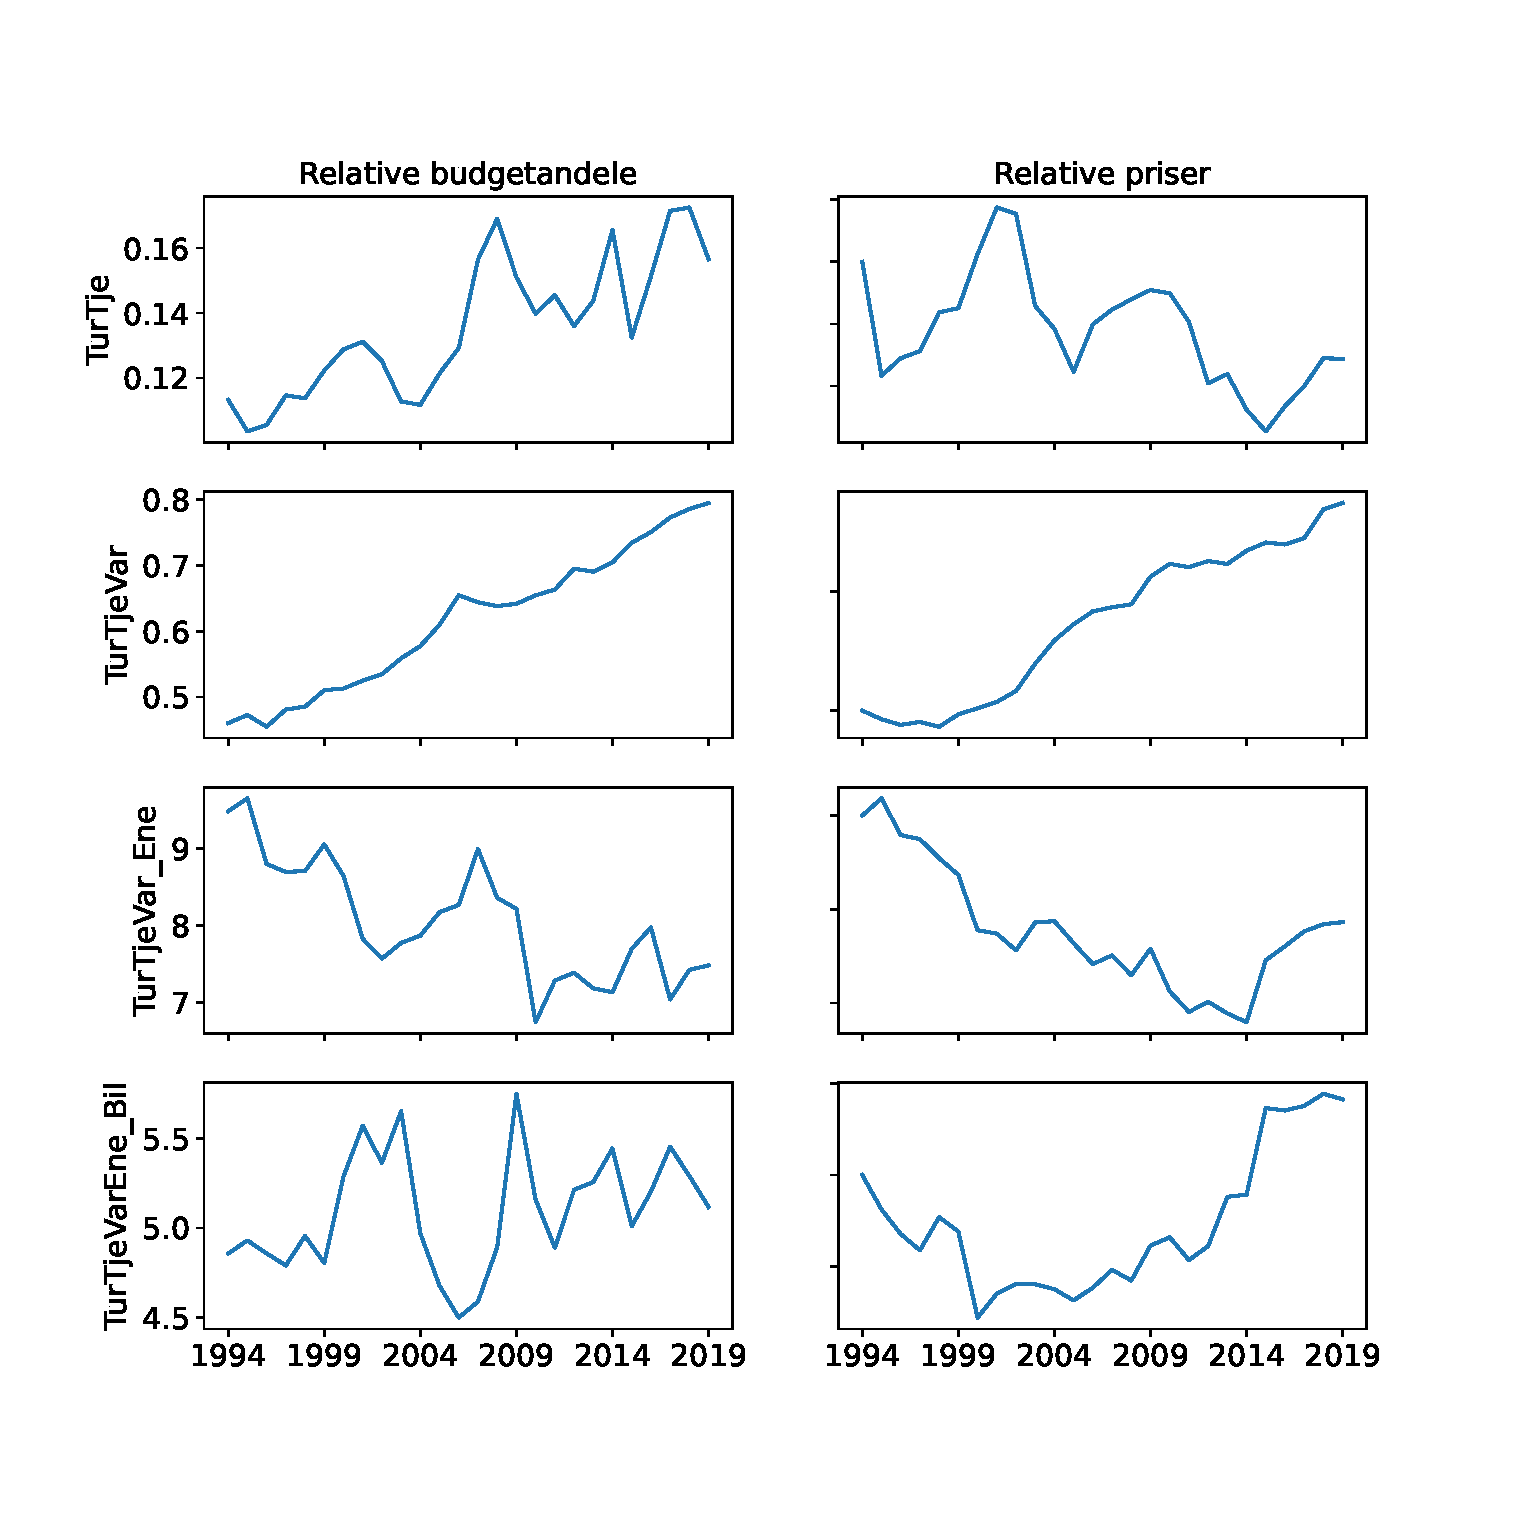
\includegraphics[width=\textwidth]{Figures/relbudrelp.eps}
\captionsetup{singlelinecheck=off,size=scriptsize}
\setlength{\captionmargin}{10pt}
\caption*{
\textbf{Note:} Nest structure\\}
\end{figure}

\subsection{Model}
Consumers $i=1,2,...,5$ differ in their income levels. We assume that the utility  of consumer $i$ of nest $u$ at time $t$ can be described as
\begin{align}\label{utileq}
    C_{i,cu,t} = \left[\sum_j (\mu_{i,j,t} C_{i,j,t})^{\frac{\sigma_{cu,i}-1}{\sigma_{cu,i}}}\right]^{\frac{\sigma_{cu,i}}{\sigma_{cu,i}-1}},
\end{align}
with $j$ denoting the components of a given nest $cu$. For example, in the second-to-bottom nest, $j=cTourServ,cGoods$. $\mu_{i,j,t}$ is a share parameter that expresses changes in the preference for good $j$ for consumer $i$. The elasticity of substitution $\sigma_{cu,i}$ is constant for each consumer. Assuming that consumers minimize costs, the log-demand function can be written
\begin{align}\label{demandeq}
    s_{i,cu,t}= (\sigma_{cu,i}-1) \mu_{i,cu,t} + (1-\sigma_{cu,i}) p_{cu,t},
\end{align}
where $s_{i,cu,t}$ is the log of the relative budget share in nest $u$, $\mu_{i,cu,t}$ is the log of the relative time-varying share parameter and $p_{cu,t}$ is log of relative prices, which are assumed identical across income groups.\footnote{This assumption is backed by data, see table PRIS201 in StatBank} 

The implication of a change in the share parameter depends on $\sigma_{cu,i}$. If $\sigma_{cu,i}<1$, an increase in $\mu_{i,cu,t}$ (a relative increase in the preference for the first good in the nest) leads to a decrease in $s_{i,cu,t}$ (a relative decrease in the consumption of the first good in the nest). This is due to higher complementarity of the goods. If $\sigma_{cu,i}>1$, the opposite is true: an increase in $\mu_{i,cu,t}$ leads to an increase in $s_{i,cu,t}$. This highlights the importance of estimating $\mu_{i,cu,t}$ and $\sigma_{cu,i}$ simultaneously, which implies that a process for $\mu$ needs to be assumed. 

This process must allow for structural shifts, such as linear trends. For example, the relative budget share of the $cTourServ$-aggregate and $cGoods$, has been increasing linearly over the sample, implying that the preference for tourism and services has increased relative to that for goods.\footnote{Or maybe just that the Baumol-effect is in play}. There are seemingly also short-run fluctuations in the relative preferences, perhaps due to business cycles, as can be seen from the relative budget shares of the $cTourServGoodEner$-aggregate and $cCars$. To capture both effects, we decompose $\mu_{i,cu,t}= \mu_{i,cu,t}^{Structural} \mu_{i,cu,t}^{Cyclical}$, where 
\begin{align}\label{mustruceq}
    \Delta \mu_{i,cu,t}^{Structural} &= \Delta \mu_{i,cu,t-1}^{Structural} + \eta_{i,cu,t} \quad \text{and} \\ \label{mucyceq}
    \mu_{i,cu,t}^{Cyclical} &= \sum_{k=1}^p \phi_{i,cu,k}\mu_{i,cu,t-k}^{Cyclical} + \epsilon_{i,cu,t},
\end{align}
and $\eta_{i,cu,t} \sim N(0,\Sigma^{\eta}_{i,cu})$ and $\epsilon_{i,cu,t}\sim N(0,\Sigma^{\epsilon}_{i,cu})$, The number of lags, $p$, is chosen to ensure no autocorrelation of $\epsilon_{i,cu,t}$ and $\phi_{i,cu,k} \in [-0.9,0.9]$ is restricted. Thus, $\mu_{i,cu,t}^{Structural}$ describes structural shifts in the preferences for consumption components, where $\mu_{i,cu,t}^{Cyclical}$ describes cyclical changes in preferences. The sluggishness of $\mu_{i,cu,t}$ depends on the ratio
\begin{align}
    \lambda = \frac{\Sigma^{\epsilon}_{i,cu}}{\Sigma^{\eta}_{i,cu}},
\end{align}
where $\lambda \rightarrow \infty$ corresponds to an assumption of a linear trend and $\lambda \rightarrow 0$ corresponds to all changes in relative budget shares are due to structural preference shifts. 

As opposed to \cite{CESkalmanmethod}, we do not use an error-correction model, as consumption is a flow variable and, from a theoretical view, should adjust quickly to changes in prices. 

\subsection{The model as a state space model}
To ease the interpretation of the Kalman filtering, we rewrite our model as a linear state space model \cite[p. 43]{durbin2012time}, which is described as
\begin{align}
    y_t &= Z_t \alpha_t + \epsilon_t, \quad &\epsilon_t \sim N(0,H_t) \\ 
    \alpha_{t+1 } &= T_t \alpha_t + R_t \eta_t  \quad &\eta_t \sim N(0,H_t),
\end{align}
where $y_t$ is the observation vector and $\alpha_t$ the state vector. 

Then, we rewrite the model described by equations (\ref{demandeq})-(\ref{mucyceq}) to the linear state space form, such that
\begin{align}
    y_t = s_t , \quad Z_t = \begin{pmatrix} p_t & 1 & 1 & 0 \end{pmatrix}, \quad \alpha_t = \begin{pmatrix} 1-\sigma \\ (\sigma-1) \mu^c_t   \\ (\sigma-1) \mu^s_t \\ (\sigma-1) \Delta \mu^s_t \end{pmatrix}, H_t = 
\end{align}


\subsection{OLS estimations of LES}
We estimate the following model for goods $c=1,2,...,44$ over time $t=1994,1995,...2019$ for different households. Prices are identical across households.
\begin{align}
    q_{ct} = \delta + \gamma t + \beta_p p_{ct} + \beta_{inc} \text{realinc}_t + \beta_{lag} q_{c,t-1} + \epsilon_t
\end{align}

A problem that arises is that the marginal budget shares are often negative. But this estimation is also kind of faulty. It estimates price and income elasticities one good at a time, instead of taking advantage of the other goods.
\newpage

\begin{landscape}
\input{tables/OLStable}
\end{landscape}
